\begin{savequote}[0.55\linewidth]
	``If you think you've seen this movie before, you are right. Cloud computing is based on the time-sharing model we leveraged years ago before we could afford our own computers. The idea is to share computing power among many companies and people, thereby reducing the cost of that computing power to those who leverage it. The value of time share and the core value of cloud computing are pretty much the same, only the resources these days are much better and more cost effective.''
	\qauthor{\textasciitilde David Linthicum, author of Cloud Computing and SOA Convergence in Your Enterprise: A Step-by-Step Guide}
\end{savequote}

\chapter{Inleiding}
\label{chap:intro}

Het onderzoek naar nieuwe cloud resource allocatieschema's staat niet stil. Elk jaar worden er nieuwe schema's ontwikkeld en gevalideerd met behulp van een simulator en/of een fysiek cloud testbed. Een belangrijke opmerking hierbij is dat niet elk nieuw schema wordt uitgetest op een fysiek cloud testbed wegens de complexiteit en de kostprijs. Hierdoor komen verborgen constanten van een fysiek cloud testbed niet aan het licht en dat heeft mogelijks een grote invloed op de performantie van het nieuwe schema. In deze masterproef wordt daarom dieper ingegaan op het bieden van een zo goedkoop mogelijk alternatief om deze nieuwe schema's te testen in een OpenStack~\cite{OpenStack2017} cloud-omgeving. Met behulp van DevStack~\cite{OpenStack2017a} wordt een OpenStack cloud-omgeving uitgerold waarbij een bestaand resource allocatiechema wordt ingeplugd met de \textit{nova scheduler} in plaats van het standaard meegeleverde schema van OpenStack zelf. Dankzij Rally~\cite{OpenStack2017b} en een Node.js-agent kunnen de gecreëerde instanties gemonitord worden waardoor de hele testopstelling uiteindelijk de mogelijkheid biedt om nieuwe allocatieschema's te evalueren in een reëele OpenStack cloud-omgeving.

\section{Wat is cloud computing?}
\label{sec:what_is_cloud_computing}

Wat is de cloud? Waar is de cloud? Zijn we in de cloud? Dit zijn allemaal relevante vragen want de term \textit{cloud computing} is overal~\cite{Griffith2016}.
Het cloud computing paradigma beschrijft applicaties waarbij toegang gebeurt via het internet en die een \textit{pool van resources} delen met andere applicaties en/of toepassingen. De eigenlijke term cloud computing verwijst naar applicaties die beschikbaar zijn via het internet alsook naar de hardware- en softwaresystemen in verschillende datacenters die deze applicaties hosten~\cite{Jennings2015}.

In een cloud-omgeving zijn er steeds drie belangrijke stakeholders die vervuld worden. Ten eerste zijn er de \textit{cloud providers}, organisaties die fysieke en virtuele servers verhuren aan andere organisaties, bedrijven, etc. Vervolgens zijn er de \textit{cloud-gebruikers} die een omgeving huren van een cloud provider om zo een dienst aan de volgende categorie te bieden. De laatste categorie beschrijft de \textit{eindgebruikers}, ook wel de gebruikers genoemd. Ze gebruiken de aangeboden diensten van de cloud-gebruikers waardoor ze een werklast genereren. Een schematisch overzicht wordt weergegven in Figuur~\ref{fig:cloud_rollen}. Een mooi voorbeeld van de drie rollen en hun onderlinge overeenkomsten is Netflix. Netflix is een cloud-gebruiker die een cloud omgeving afhuurt van een grote organisatie zoals bijvoorbeeld Google of Amazon (de cloud providers). De mensen thuis (eindgebruikers) kijken naar verschillende series, films, etc. waardoor ze op hun beurt werklast genereren voor de servers die Netflix huurt.

De drie stakeholders van cloud-computing hebben elk hun kosten. Cloud providers betalen de kosten om infrastructuur aan te kopen en deze te onderhouden waarna ze deze infrastructuur meestal aanbieden via een pay-as-you-go schema aan de cloud-gebruikers. Cloud-gebruikers daarentegen factureren vaak vaste maandelijkse bedragen aan hun eindgebruikers waardoor het efficiënt gebruiken van resources zeer belangrijk is zodat hun eigen kosten aan de cloud providers gedekt worden.

\begin{figure}
	\centering
	\begin{subfigure}{\textwidth}
		\centering
		\centerline{
			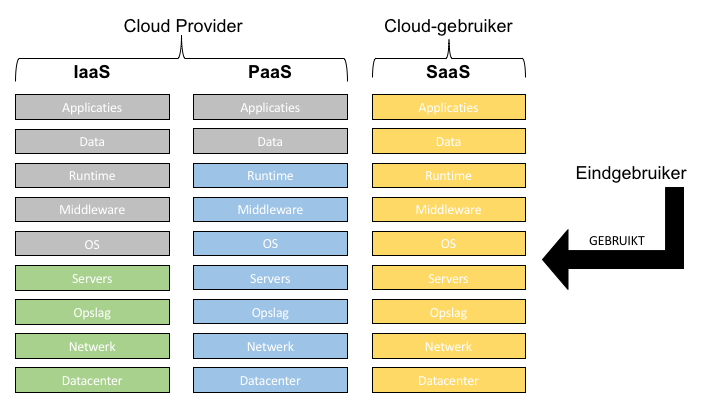
\includegraphics[scale=0.47]{cloud_rollen}
		}
	\end{subfigure}
	\caption{Cloud stakeholders met de bijhorende cloud-vorm}
	\label{fig:cloud_rollen}
\end{figure}

\subsection{Tenants en \textit{multi-tenancy}}

Multi-tenancy betekent dat er verschillende aanvragen van verschillende organisaties of bedrijven (tenants) concurrent behandeld worden door 1 of meerdere instanties van de applicatie die de hardware- en software-infrastructuur met elkaar delen~\cite{Guo2007}. Een tenant wordt dus voorgesteld als een eindgebruiker die een deel van de cloud-applicatie wenst te gebruiken, al dan niet gedeeld met andere tenants. Hierbij moet de cloud-applicatie zo ontwikkeld worden dat deze multi-tenancy ondersteunt. Cloud computing zelf is een vorm van multi-tenancy aangezien verschillende gebruikers dezelfde infrastructuur met elkaar delen.

\subsection{Service Level Agreement}

Een Service Level Agreement (SLA) is een belangrijk onderdeel in de wereld van cloud computing. Het is een overeenkomst tussen twee verschillende partijen die dienst doet als blauwdruk en garantie biedt over de aangeboden diensten~\cite{Wired2017}. Zo sluit bijvoorbeeld een cloud provider een SLA af met een cloud-gebruiker en sluit een cloud-gebruiker een SLA af met de eindgebruikers. Een SLA kan beschouwd worden als een reeks van verwachtingen en criteria waardoor geen van beide partijen voor verrassingen komen te staan bij eventuele wijzigingen, zowel verwachte als onverwachte, in de cloud service. Een aantal voorbeelden van deze criteria zijn beschikbaarheid (99.95\% \textit{uptime}), performantie, beveiliging, \textit{data recovery}, locatie van de data, etc. Dankzij zo'n SLA kan een gebruiker de meest geschikte (beste prijs/kwaliteit afhankelijk van de noden) cloud-oplossing kiezen, want niet elke gebruiker heeft een zeer betrouwbaar en duur systeem nodig.

\section{Probleemstelling en doel van de masterproef}
\label{sec:problem}

Er zijn al meerdere nieuwe technieken ontwikkeld om cloud resources te alloceren en deze worden samengevat in Sectie~\ref{sec:newcras}. Een belangrijk detail dat hierbij nog niet vermeld is: iets minder dan de helft van deze nieuwe methoden zijn enkel getest in simulators en dus niet in echte cloud omgevingen zoals we zullen zien in Tabel~\ref{tab:resallocschemes} van Hoofdstuk~\ref{sec:newcras}. Deze kolom geeft aan of het nieuwe schema getest is op een echte cloud-omgeving of met behulp van een simulator en de verdeling is respectievelijk 16 schema's en 13 schema's. Een mogelijke belangrijke reden hiervoor is de zeer hoge kostprijs bij eventuele fouten in de methode zoals vermeld in de inleiding van Hoofdstuk~\ref{chap:intro}. Stel dat een onderzoeker zijn nieuwe methode wil uittesten in een gehuurde Microsoft Azure omgeving dan kunnen de kosten zeer hoog uitvallen indien er bijvoorbeeld te veel resources worden aangevraagd door een fout in de methode.

Het doel van deze thesis is het mogelijk maken om nieuwe methoden te testen op een kleinschalige OpenStack cloud-omgeving. Met behulp van Nova en de Orchestration-services van OpenStack kan een nieuwe methode eenvoudig en snel worden getest. Via de Nova-scheduler kan het nieuwe schema worden ingeplugd en met behulp van de Orchestration-services kan een schaalbare applicatie horizontaal schalen. Dit zorgt voor een zware werklast op de cloud-omgeving waarbij de verschillende hosts gemonitord zullen worden. Ten slotte worden de verkregen resultaten geëvalueerd met nadien een eventuele vergelijking tussen deze resultaten en de resultaten van een simulatortest.

Om de werking van dit alles uit te leggen zal een \textit{proof-of-concept} worden uitgewerkt met een eenvoudig schema.
Allereerst zal het eenvoudig schema, Round Robin, worden ingeplugd in Nova. Vervolgens zal een schaalbare applicatie, namelijk FaaFo (First App Application For OpenStack) worden uitgerold op de ontwikkelde OpenStack-omgeving. Daarna zal, door een stijgende, gegenereerde werklast de applicatie horizontaal geschaald worden dankzij de Orchestration-services van OpenStack. De verschillende hosts worden hierbij gemonitord om te kijken of de werklast verdeeld werd zoals gewenst.

Het vervolg van deze masterproef wordt als volgt ingedeeld. In het volgende hoofdstuk wordt er dieper ingegaan op de termen resource-allocatie en OpenStack. Daarna wordt het relevant werk besproken dat een mogelijke leidraad kan bieden. Vervolgens beschrijft Hoofdstuk 3 de testomgeving en hoe deze tot stand is gebracht waarna Hoofdstuk 4 de verschillende mogelijkheden om te monitoren toelicht samen met de gekozen manier. Hoofdstuk 5 legt de manier waarop de evaluaties gebeuren uit met de bijhorende proof-of-concept. Ten slotte worden in Hoofdstuk 6 de besluiten geformuleerd, gevolgd door de bibliografie en enkele bijlagen.